% Slide 7 | Results E4 | M1 (Lakshya Satya) | 2:00 | the perfect pair
\begin{frame}{E4: a perfect pair earns only about half its theory}
\framesubtitle{Slide 7 \textbullet\ Results E4 \textbullet\ Lakshya \textbullet\ 2:00}
\vspace{-2pt}
\begin{columns}[T,onlytextwidth]
\column{0.58\textwidth}
  \centering
  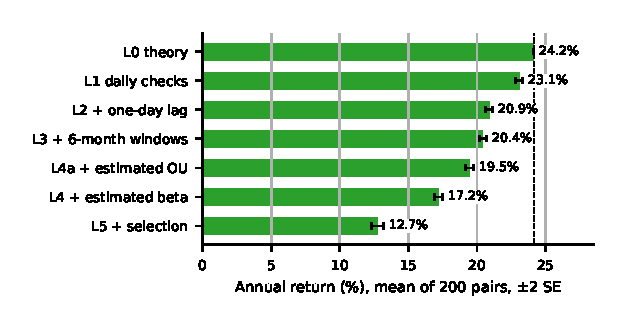
\includegraphics[width=\linewidth]{fig_e4_synthetic_report}
\column{0.38\textwidth}
  \small\raggedright
  A made-up pair that follows the OU model exactly, 200 runs through the real pipeline:
  \begin{itemize}\setlength{\itemsep}{3pt}
    \item theory \textbf{24.2\%} a year
    \item pipeline \textbf{12.7\%}
    \item biggest loss: picking the pair, $-4.5$ points
  \end{itemize}
\end{columns}
\pairTakeaway{The selection test finds this genuine pair in only 74\% of windows.}
\end{frame}
